\section{A patch-based heat equation solver}


\chapterDescription
  {
    60 minutes.
  }
  {
    Chapter \ref{chapter:quickstart}.
  }

In this section, we sketch how to realise a simple explicit heat equation
solver that is based upon patches.
The idea is that we embed a small regular Cartesian grid into each individual
spacetree leaf.
This patch is surrounded by a halo/ghost cell layer holding copies from
neighbouring patches.

\begin{center}
  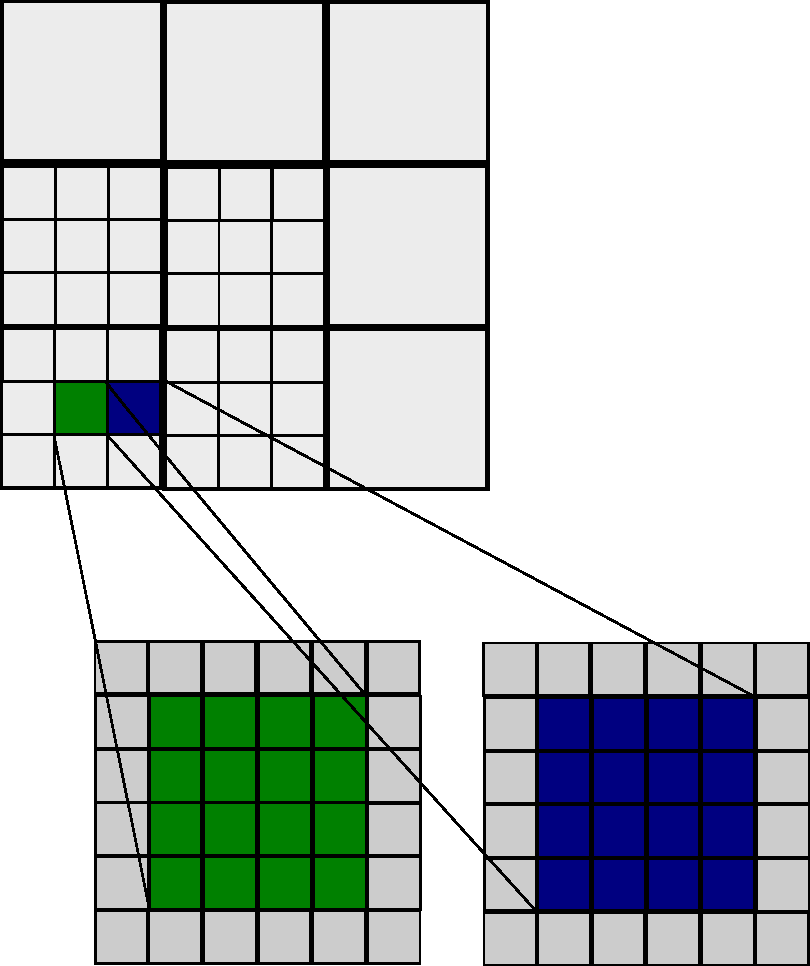
\includegraphics[width=0.4\textwidth]{44_patch-based-solver/patches.pdf}
\end{center}

In the sketch, we enbed $4\times 4$ patches into the spacetree cells.
Two cells (blue and green) are illustrated.
Each patch is surrounded by a halo layer of size one.
We will write the code to work within the patches, while the layers around the
patches will hold copies of the neighbouring patches and thus couple them.

For this endeavour, we need the toolbox \texttt{multiscalelinkedcell} that you
can download from the Peano webpage.
We assume that the whole toolbox is unzipped into a directory
\texttt{multiscalelinkedcell} which is held by your source directory.


\subsection{Preparation}

We start with the creation of a file \texttt{PatchDescription.def} in your
project's root directory. 
In our example, each patch solely shall hold one array of unknowns $u$ that are
associated to the vertices of the patch.
So each patch will have exactly $(4+2+1)^2$ unknowns (the four is the size,
there's two halo cells along each coordinate axis, and then there's finally one
more vertex than there are cells).
Besides the unknowns called $u$, we also store the position and size as well as
the level with each patch---well-aware that level and size are kind of
redundant.

\begin{code}
#include "peano/utils/Globals.h"

Packed-Type:  int;

Constant: DIMENSIONS;

/**
 * A cell description describes one individual patch of the overall grid, i.e. 
 * it holds pointers to the actual data of the patch (arrays) and its meta data
 * such as time stamps. Each unrefined node of the spacetree, i.e. each leaf, 
 * holds exactly one instance of this class. 
 */
class myprojectname::records::PatchDescription {
  /**
   * Two pointers to float arrays.
   */
  parallelise persistent int     u;
  /**
   * I need level and offset to be able to determine the source and image in 
   * the adaptive case.
   */
  parallelise persistent int     level;
  parallelise persistent double  offset[DIMENSIONS];
  parallelise persistent double  size[DIMENSIONS];
};
\end{code}

Please note that $u$ is modelled as integer. 
Actually, we do not hold the data directly within the patch description but we
make the patch description hold a pointer to the actual data.
The data will be managed by Peano on the heap. 
The heap uses integers as pointers.
They are actually hash map indices.


Our system design is as follows:
\begin{itemize}
  \item Each cell holds a pointer to one \texttt{PatchDescription}.
  \item The \texttt{PatchDescription} holds a pointer to the actual patch data
  and comprises some additional meta data (such as the level).
  \item Each vertex holds $2^d$ pointers to the
  \texttt{PatchDescription} instances belonging to the adjacent cells.
\end{itemize}


Whenever we enter a cell, we can thus take its patch description, and get the
actual data from this description.
Alternatively, we can use the cell's $2^d$ adjacent vertices. 
As they know the adjacent patch descriptions, we can also get the data
associated to cell neighbours and thus befil the ghost layers, e.g.


Take the Peano description file of our project ensurte that it contains the
following lines:
\begin{code}
heap-dastgen-file: PatchDescription.def

[...]

vertex:
  dastgen-file: Vertex.def
  read vector2PowD(int): PatchIndex
  write vector2PowD(int): PatchIndex
  
[...]

event-mapping:
  name: Mapping1


event-mapping:
  name: Mapping2
  
[...]

adapter:
  name: Adapter1
  merge-with-user-defined-mapping: Mapping1
  merge-with-predefined-mapping: MultiscaleLinkedCell(PatchIndex)

adapter:
  name: Adapter2
  merge-with-user-defined-mapping: Mapping2
  merge-with-predefined-mapping: MultiscaleLinkedCell(PatchIndex)
\end{code}

Managing all the adjaceny data (making each vertex point to the right patch)
obviously is a tedious task.
The \texttt{multiscalelinkedcell} toolbox fortunately does most of the stuff for
us, if we augment each adapter with a predefined mapping, tell this mapping what
the attribute for the patch handling will be (\texttt{PatchIndex}), and augment
the vertex accordingly. 
Finally, open \texttt{Vertex.def} and augment it accordingly:

\begin{code}
#include "peano/utils/Globals.h"

Packed-Type:  int;

Constant: TWO_POWER_D;

class myprojectname::dastgen::Vertex {
  /**
   * These guys are pointers to the adjacent cells. Actually, they do not point 
   * to the neighbouring cells but to the heap indices associated to these cells.
   * These heap indices reference one or several instances of PatchDescription.
   */
  expose persistent int patchIndex[TWO_POWER_D];  
  
  [...]
};
\end{code}

We run the translation process and add the toolbox directory to the PDT call:
\begin{code}
 java -jar <mypath>/pdt.jar <mypath>/project.peano-specification <mypath> \
 <mypath>/usrtemplates:<mypath>/multiscalelinkedcell
\end{code}


The PDT in collaboration with the toolbox will now create code that makes each
vertex track the \texttt{patchIndex} value of the adjacent cells.
If you change your grid, the indices are updated automatically, as long as you
merge \texttt{MultiscaleLinkedCell} into your adapters.
To make the code compile, you finally have to add a routine 
\begin{code}
  int getPatchIndex() const;
\end{code}
to your Cell class. 
Make the routine return the value of an attribute \texttt{persistent int 
patchIndex} that you add to your \texttt{Cell.def}.
Set this field to -1 in the default constructor.

\subsection{Setting up the patches}

Before we start any coding, we have to specify which heaps we want to use to
administer the patch description objects and the actual $u$ data.
One option is to define this centrally in the \texttt{Cell.h} file that is
generated by the PDT:
\begin{code}
#include "peano/heap/Heap.h"
#include "<mypath>/records/PatchDescription.h"

namespace myprojectsnamespace { 
  class Cell;
  
  typedef peano::heap::PlainHeap< myprojectsnamespace::records::PatchDescription >  
    PatchDescriptionHeap;
  typedef peano::heap::PlainDoubleHeap                                    DataHeap;
}
\end{code}

\noindent
In this setup, we use the plain heap from Peano's heap directory to administer
both the data and the patch descriptions. 
There are several other, more sophisticated, heap implementations available. 
While they allow you to tune your code for special purposes, the plain heap
typically is a good starting point.

To set up the patches, we create plug into the mapping creating our grid. 
Alternatively, we can first create the grid and then outsource the patch
initialisation into an additional mapping.
In any case, I strongly encourage you to initialise the heap as a first step. 
This is however optional: 
\begin{code}
void myprojectsnamespace::mappings::InitPatches::beginIteration(
  ...
) {
  logTraceInWith1Argument( "beginIteration(State)", solverState );

  PatchDescriptionHeap::getInstance().setName( "patch-description-heap" );
  DataHeap::getInstance().setName( "data-heap" );

  logTraceOutWith1Argument( "beginIteration(State)", solverState);
}
\end{code}
So far, each cell points to index -1 as patch description index, and each vertex
knows that all adjacent cells point to -1. We change this now as we plug into 
\texttt{enterCell} and introduce a new operation in Cell:

\begin{code}
void myprojectsnamespace::mappings::InitPatches::enterCell(
  ...
) {
  fineGridCell.init( ... ); // please pass through the level, the offset and the size
}


void myprojectsnamespace::Cell::initCellInComputeTree( ... ) {
  const int newPatchIndex = PatchDescriptionHeap::getInstance().createData(1);
  _cellData.setPatchIndex( newPatchIndex );
  assertion( newPatchIndex>=0 );
  ...
}

\end{code}

\noindent
We finally befill the patch data, i.e.~replace the dots in
\texttt{initCellInComputeTree}.
This is a three-fold process.
First, we initialise all the meta data.
Second, we create the real patch. 
Finally, we make the meta data record point to this data, while 
the cell itself points to the \texttt{PatchDescription} instance.
 
\begin{center}
  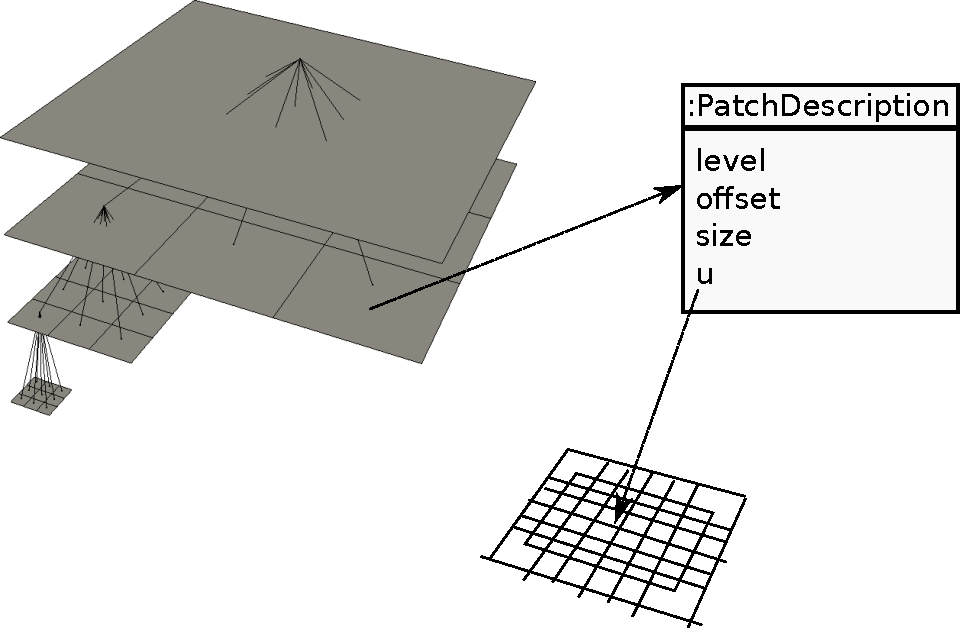
\includegraphics[width=0.5\textwidth]{44_patch-based-solver/data.pdf}
\end{center}

\noindent
It is up to you to specificy the semantics of the data arrays used. 
They can represent overlapping or non-overlapping patches.
It just has paid off not to make any overlap exceed any neighbouring cell on the
same level.
The introductory sketch of this chapter illustrates $4\times 4$ patches with a
ghost layer/overlap of one. 
A code for this setup might read as follows:

\begin{code}
void myprojectsnamespace::Cell::initCellInComputeTree( ... ) {
  const int numberOfPatchDescriptionsPerCell = 1;
  const int newPatchIndex = PatchDescriptionHeap::getInstance().createData
    (numberOfPatchDescriptionsPerCell);
  _cellData.setPatchIndex( newPatchIndex );
  assertion( newPatchIndex>=0 );

  records::PatchDescription patchDescription =
    PatchDescriptionHeap::getInstance().getData(newPatchIndex)[0]; 
  
  patchDescription.setU( DataHeap::getInstance().createData(7*7) );
  patchDescription.setLevel(...);
  patchDescription.setOffset(...);
  patchDescription.setSize(...);
}

\end{code}


\begin{remark}
  There is absolutely no reason to restrict a code to use only the finest level
  of the spacetree. Furthermore, it might make sense to use different patch
  sizes in different cells of the same level. Please note that all the patch
  techniques also work if you store higher order DG shape functions in your
  cells, e.g.
\end{remark}



\subsection{Working with patches on regular grids}

As each cell points to patch description through its field \texttt{PatchIndex},
it is a natural choice to work with the associated patch data in
\texttt{enterCell}.
Before we actually do the work, we use the data from the 
\texttt{PatchIndex} objects of the neighbouring cells to initialise our ghost
cells.
In our case, a simple copying does the job. In other situations, you might have
to implement more sophisticated projection operators.

\begin{code}
#include "multiscalelinkedcell/HangingVertexBookkeeper.h"
#include "multiscalelinkedcell/SAMRTools.h"
#include "peano/utils/Loop.h"
...
void pesplines::mappings::JacobiUpdate::enterCell( ... ) {
 if (
  !fineGridCell.isRefined()
  &&
  multiscalelinkedcell::HangingVertexBookkeeper::allAdjacencyInformationIsAvailable(
   VertexOperations::readPatchIndex(fineGridVerticesEnumerator,fineGridVertices)
  )
 ) {
  intialiseGhostLayerOfPatch(
    fineGridCell,
    fineGridVertices,
    fineGridVerticesEnumerator
  );
   
  solve(
    PatchDescriptionHeap::getInstance().getData( fineGridCell.getPatchIndex() )[0],
    fineGridVerticesEnumerator.getCellSize()
  );
 }  
}
\end{code}

\noindent
The use of the predicate \texttt{allAdjacencyInformationIsAvailable} is too
careful here: it should always return \texttt{true}.
In dynamically adaptive settings, it can happen that adjacency information in
the vertices (i.e.~which patch descriptions are held by the adjacent cells) it
not up-to-date immediately.
In such a case, the branching would skip a cell with incomplete data and wait
for the next traversal where all information is available.


The initialisation of the ghost layer uses Peano's d-dimensional loops (the
code then should work for $d=3$ as well), it rather technical, but not too
difficult to understand as it realises plain copying at the end of the day.
Again, we use operations provided by the \texttt{multiscalelinkedcell} package:

\begin{code}
void pesplines::mappings::MatVec::intialiseGhostLayerOfCell(
 Cell&                                 fineGridCell,
 Vertex * const                        fineGridVertices,
 const peano::grid::VertexEnumerator&  fineGridVerticesEnumerator
) {
 const tarch::la::Vector<THREE_POWER_D,int> neighbourCellIndices = 
  multiscalelinkedcell::getIndicesAroundCell(
   VertexOperations::readPatchIndex(fineGridVerticesEnumerator,fineGridVertices)
 );

 assertion3(
   multiscalelinkedcell::HangingVertexBookkeeper::allAdjacencyInformationIsAvailable(
    VertexOperations::readPatchIndex(fineGridVerticesEnumerator,fineGridVertices)
   ),
   fineGridVerticesEnumerator.toString(),
   VertexOperations::readPatchIndex(fineGridVerticesEnumerator,fineGridVertices),
   neighbourCellIndices
 ); // no enty of neighbourCellIndices points to a patch description on the
    // heap that does not exist
 
 // we take data from surrounding patches and always write into the
 // patch in the center (destPatchDescription)
 records::PatchDescription& destPatchDescription = 
  PatchDescriptionHeap::getInstance().getData( fineGridCell.getPatchIndex())[0];

 dfor3(i)
  // i does not point to the central patch (all entries 1) and is valid
  // i.e. we are not at the domain boundary, e.g.
  if (
   i!=tarch::la::Vector<DIMENSIONS,int>(1) &&
   neighbourCellIndices(iScalar) > 
    multiscalelinkedcell::HangingVertexBookkeeper::InvalidAdjacencyIndex
  ) {
   assertion(neighbourCellIndices(iScalar)>=0);
   records::PatchDescription& srcPatchDescription 
    = PatchDescriptionHeap::getInstance().getData( neighbourCellIndices(iScalar) )[0];
 
   // this if is always true as long as we work with a regular grid
   if (srcPatchDescription.getLevel()==destPatchDescription.getLevel()) {
    // so now write your well-suited for loop here that befill all entries 
    // of the ghost layer of your patch. If the for loop determines the 
    // indices destVertexIndex and srcVertexIndex specifying vertices within 
    // the patch, then the loop body copying the data around reads as 
    DataHeap::getInstance().getData(destPatchDescription.getU())
      [destVertexIndex]._persistentRecords._u =
     DataHeap::getInstance().getData(srcPatchDescription.getU())
      [srcVertexIndex]._persistentRecords._u;
   }
  }
 enddforx // counterpart of dfor3 (see documentation in source code)
}
\end{code}

\noindent
The texttt{dfor3(i)} runs over a $\{0,1,2\}^d$ domain.
In the loop body (that has to be terminated by a \texttt{enddforx} pragma), it
provides two loop counters: \texttt{i} is a d-dimensional integer vector where
each entry is from $\{0,1,2\}$.
Furthermore, it gives us another loop counter \texttt{iScalar} which runs from 0
through $3^d-1$, i.e.~is a linearisation of \texttt{i}.
All the macros are defined in \texttt{Loop.h}.


\texttt{getIndicesAroundCell} is a helper function that takes the $2^d$ adjacent
vertices of a cell.
It actually requires their \texttt{PatchIndex} entries which are automatically
set by the predefined mapping.
The helper tool returns an array with $3^d$ entries to be read as a $3^d$
integer field.
The first entry holds the patch index of the left bottom neighbour.
The second entry holds the patch index of the bottom neighbour.
The fourth entry holds the patch index of the left neighbour.
The fifth entry hold the patch index of the cell itself.
And so forth.
The operation works for any dimension.
Study its source code documentation for details.


How the actual copying is done depends on the semantics of your data. 
It also depends on column-major or row-major storage formats for the patch data.
The implementation of the actual \texttt{solve} operation then finally is
straightforward: take the $u$-array and run through it. Again, a \texttt{dfor}
loop might simplify your code.
If you struggle with the \texttt{solve} operation, it might make sense to study
the plotting in the next section first. 
It uses exactly the sketched loop of the patch entries.


\begin{remark}
  It is not clear a priori whether it is better to have overlapping patches or
  non-overlapping data structures. With overlaps, there's an additional memory
  overhead for redundant data and data has to be moved around in the preamble of
  \texttt{enterCell}, e.g. In return, the actual work on the patches can be
  realised on a continuous array; and thus benefit from vectorisation and
  parallel fors. Alternatively, one can not use any redundant data and instead
  access the neighbouring data indirectly. This makes the actual computation
  often more complicated (one has to analyse whether data is held within the
  patch of comes from an adjacent patch), but induces no memory overhead and
  perhaps reduces the stress on the memory subsystem.
\end{remark}



\subsection{Plotting}

We briefly sketch what rapid coding of the plotting of a patch-based solver
might look like.
For this, we rely on a mapping \texttt{Plot} that holds plotter classes from 
Peano's plotter component.


\begin{code}
#include "tarch/plotter/griddata/blockstructured/PatchWriterUnstructured.h"

namespace pesplines {
  namespace mappings {
    class Plot;
  }
}

class pesplines::mappings::Plot {
  private:
    ...
    static int                  _snapshotCounter;

    tarch::plotter::griddata::blockstructured::PatchWriter*                      _writer;
    tarch::plotter::griddata::blockstructured::PatchWriter::SinglePatchWriter*   _patchWriter;
    tarch::plotter::griddata::blockstructured::PatchWriter::VertexDataWriter*    _uWriter;
};
\end{code}

\noindent
The implementation plugs into \texttt{beginIteration} and \texttt{endIteration}
to open the plotter or to write its data into a file, respectively.
Depending on the build type, we either plot binary data or we plot a plain text
file that is easier to debug.

\begin{code}
int ...::mappings::Plot::_snapshotCounter(0);

void ...::mappings::Plot::beginIteration(
  ...::State&  solverState
) {
  #if defined(Asserts) || defined(Debug)
  _writer = new tarch::plotter::griddata::blockstructured::PatchWriterUnstructured( 
    new tarch::plotter::griddata::unstructured::vtk::VTKTextFileWriter() );
  #else
  _writer = new tarch::plotter::griddata::blockstructured::PatchWriterUnstructured( 
    new tarch::plotter::griddata::unstructured::vtk::VTKBinaryFileWriter() );
  #endif
  _patchWriter            = _writer->createSinglePatchWriter();

  _uWriter         = _writer->createVertexDataWriter("u",3);
}


void ...::mappings::Plot::endIteration(
  ...::State&  solverState
) {
  _patchWriter->close();
  _uWriter->close();

  delete _uWriter;
  delete _patchWriter;

  _uWriter = 0;
  _patchWriter = 0;

  std::ostringstream snapshotFileName;
  snapshotFileName << "solution"
                   #ifdef Parallel
                   << "-rank-" << tarch::parallel::Node::getInstance().getRank()
                   #endif
                   << "-" << _snapshotCounter
                   << ".vtk";
  _writer->writeToFile( snapshotFileName.str() );

  _snapshotCounter++;

  delete _writer;
  _writer = 0;
}
\end{code}

\noindent
The heart of the plotting can be found in \texttt{enterCell} where the
actual patch data it piped into the solution plotter:


\begin{code}
void ...::mappings::Plot::leaveCell(...) {
 if ( !fineGridCell.isRefined() ) {
  assertion(PatchDescriptionHeap::getInstance().isValidIndex(fineGridCell.getPatchIndex()));
  const records::PatchDescription& patchDescription   
   = PatchDescriptionHeap::getInstance().getData( fineGridCell.getPatchIndex() )[0];

  const std::pair<int,int> indexPair = _patchWriter->plotPatch(
    fineGridVerticesEnumerator.getVertexPosition(),
    fineGridVerticesEnumerator.getCellSize(),
    4+1 // number of inner cells per spacetree leaf
  );

  int unknownVertexIndex = indexPair.first;
  //int unknownCellIndex   = indexPair.second;

  dfor(i,4+1) {
   const tarch::la::Vector<DIMENSIONS,int> currentVertex = i + 1;
   const int linearisedCurrentVertex 
    = peano::utils::dLinearisedWithoutLookup(currentVertex,4+1);
   const double u = DataHeap::getInstance().getData(patchDescription.getU())
    [linearisedCurrentVertex]._persistentRecords._u;

    _uWriter->plotVertex( unknownVertexIndex,u );
    unknownVertexIndex++;
  }
 }
}
\end{code}



\subsection{Adaptive grids}

